\RequirePackage[orthodox]{nag}
\documentclass[11pt]{article}

%% Define the include path
\makeatletter
\providecommand*{\input@path}{}
\g@addto@macro\input@path{{include/}{../include/}}
\makeatother

\usepackage{../../include/akazachk}


\title{ECH4905 ChemE Optimization HW 3}
\author{Andres Espinosa}

\begin{document}
\maketitle

\section{Problem 1}
Consider the nonlinear program
\begin{align*}
  \text{minimize} & \quad x_1^2 + 2x_2^2 \\
  \text{subject to} & \quad x_1^2 + x_2^2 \leq 5 \\
  & \quad 2x_1 - 2x_2 = 1
\end{align*}

\subsection{Part a}
Write the KKT conditions for the problem
\label{p1:kkt}

\textbf{Solution: }
%TODO: Do this 

\subsection{Part b}
Using \ref{p1:kkt} and other conditions for optimality, what can you conclude about the following solutions to the nonlinear program
\begin{align*}
  x = 
  \begin{bmatrix}
    0 \\ 0
  \end{bmatrix}
  , \quad
  x = 
  \begin{bmatrix}
    1 \\ \frac{1}{2}
  \end{bmatrix}
  , \quad 
  x = 
  \begin{bmatrix}
    \frac{1}{3} \\ -\frac{1}{6}
  \end{bmatrix}
\end{align*}

\textbf{Solution: }

\section{Problem 2}
Consider the following flowsheet:

\begin{figure}[htbp]
  \centerline{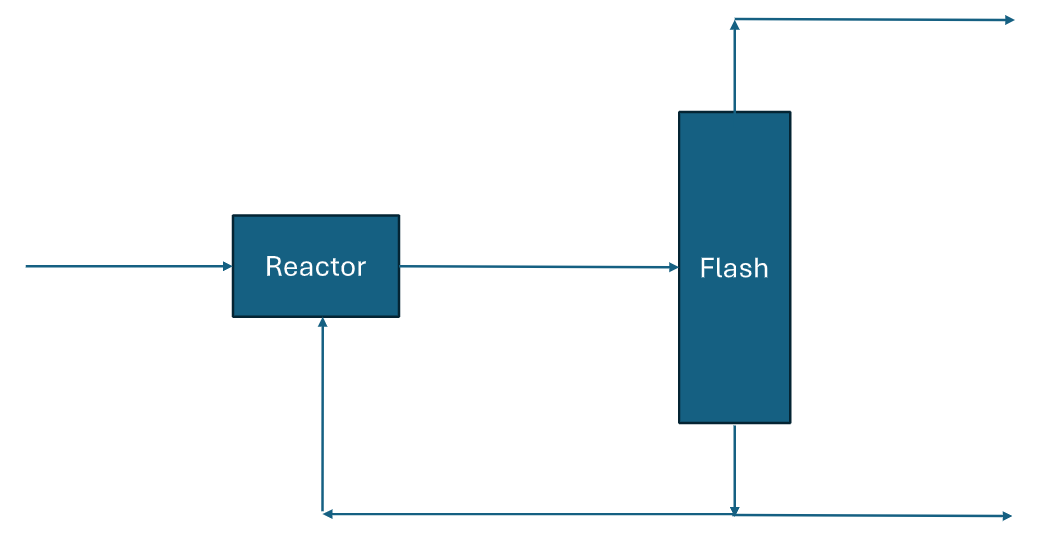
\includegraphics[width=0.5\textwidth]{images/flowsheet.png}}
  \label{fig:flowsheet}
\end{figure}

Assume that the following reaction takes place with a 50\% conversion. The feed to
the reactor consists of pure A.
\[ A \rightarrow B \]
The flash separator can be modeled as a perfect separation unit, capable of
producing any required purity.
We assume that the purge fraction should be between 1\% to 99\%.
The profit is given by the following equation:
\[ 0.5B_{\text{Top}} - 0.1F_R(500 - T) - 10^{-5}V \]
Where $B_{\text{Top}}$ is the molar flow B exiting as top product from the flash separator. 
And $F_R$ is the recycle molar flow rate.

\subsection{Part a}
Formulate a model of this process.

\textbf{Solution: }
%TODO: Formulate the model

\subsection{Part b}
Set up the model in GAMS and try 3 different NLP solvers, compare the results.

\textbf{Solution: }
%TODO: Set up the model in GAMS and compare results

\end{document}